Using the results of Problem 6 (\ref{eq:AandB}), we can implement a SIMULINK model (see figure \ref{fig:linearModelMatrix}) of the linear system.

\begin{figure}[H]
 \centering 
 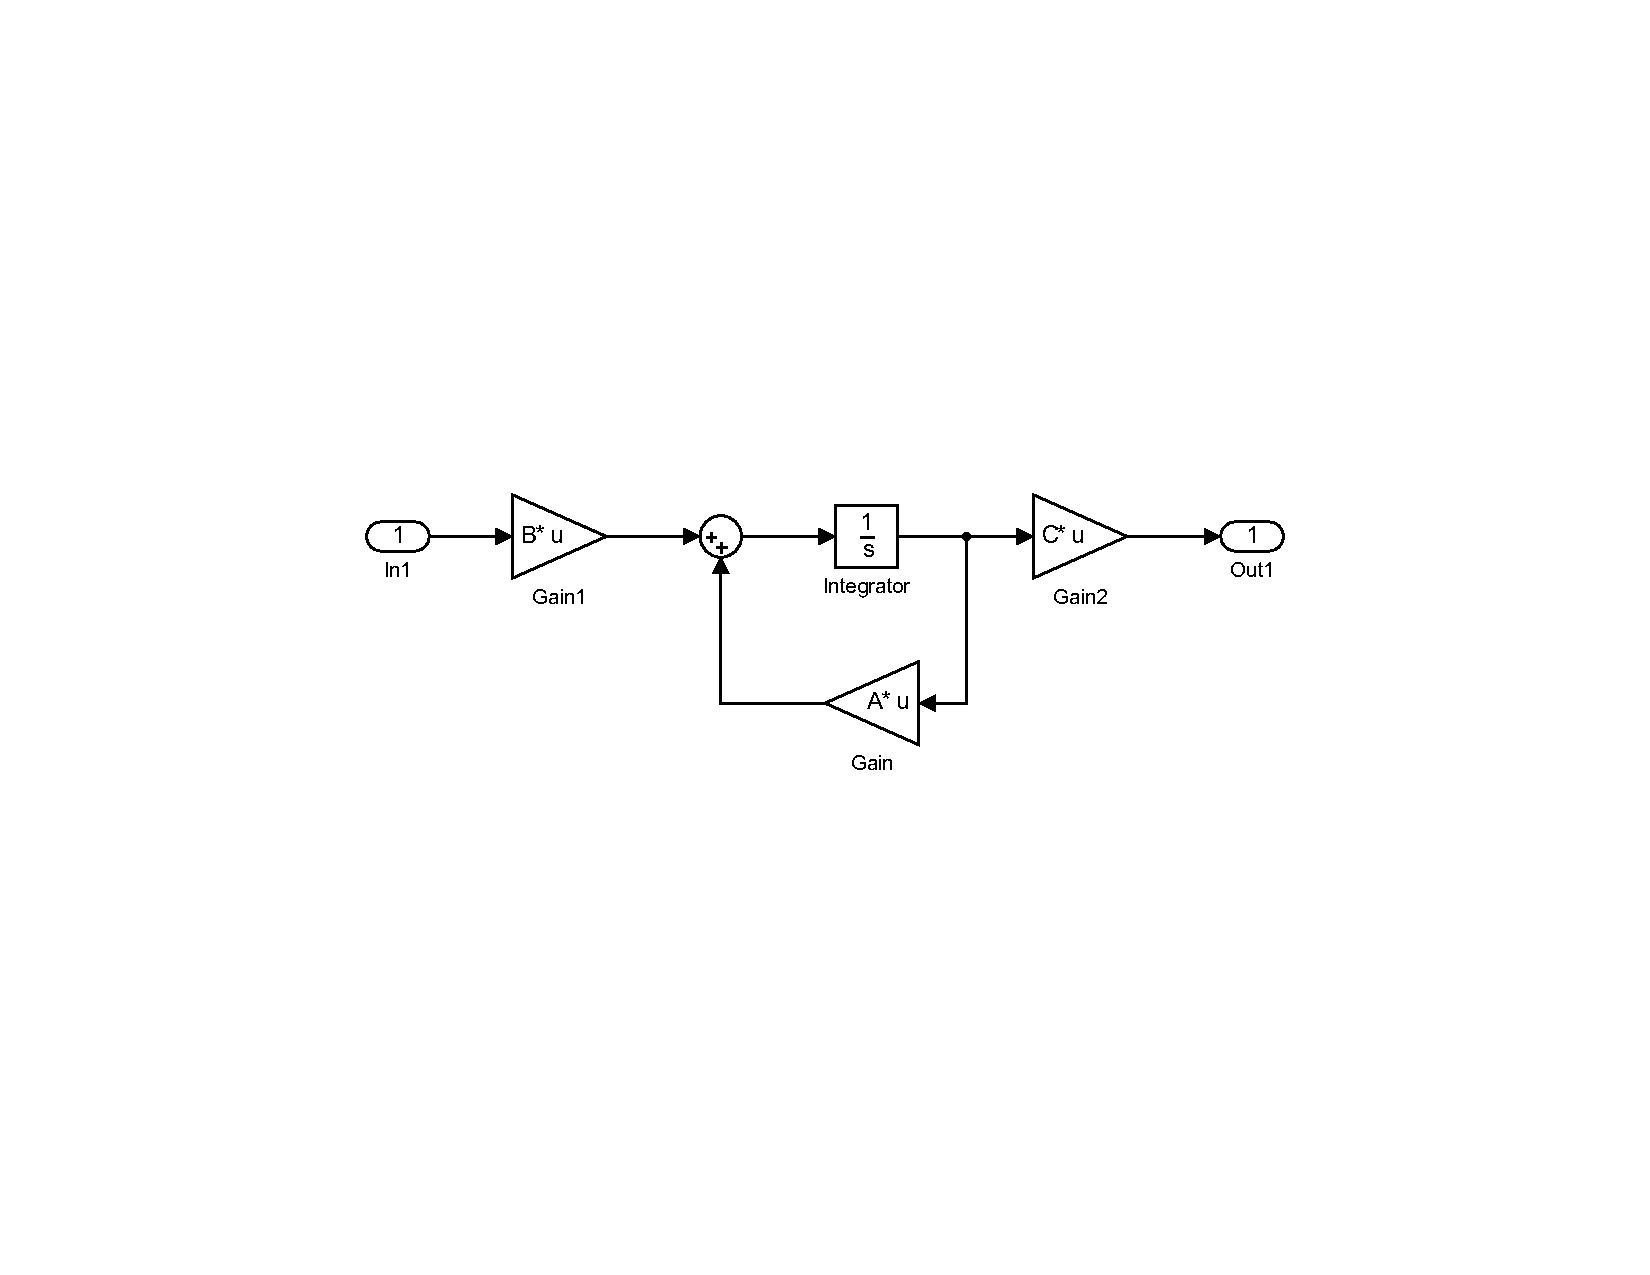
\includegraphics[trim=5cm 7cm 2cm 7cm, clip=true, totalheight=0.25\textheight, angle=0]{figures/linearModelMatrix.pdf}
 \caption{SIMULINK model of the linearised loudspeaker}
\label{fig:linearModelMatrix}
\end{figure}

Then, we can simulate the linearised model with an input $u_e=A_u\sin(2\pi f_ct)$, where $A_u=5V$ and $f_c=20Hz$. The states response in the time domain is plotted figure \ref{fig:responseLMt} and the PSD is plotted figure \ref{fig:responseLMf}.

\begin{figure}[H]
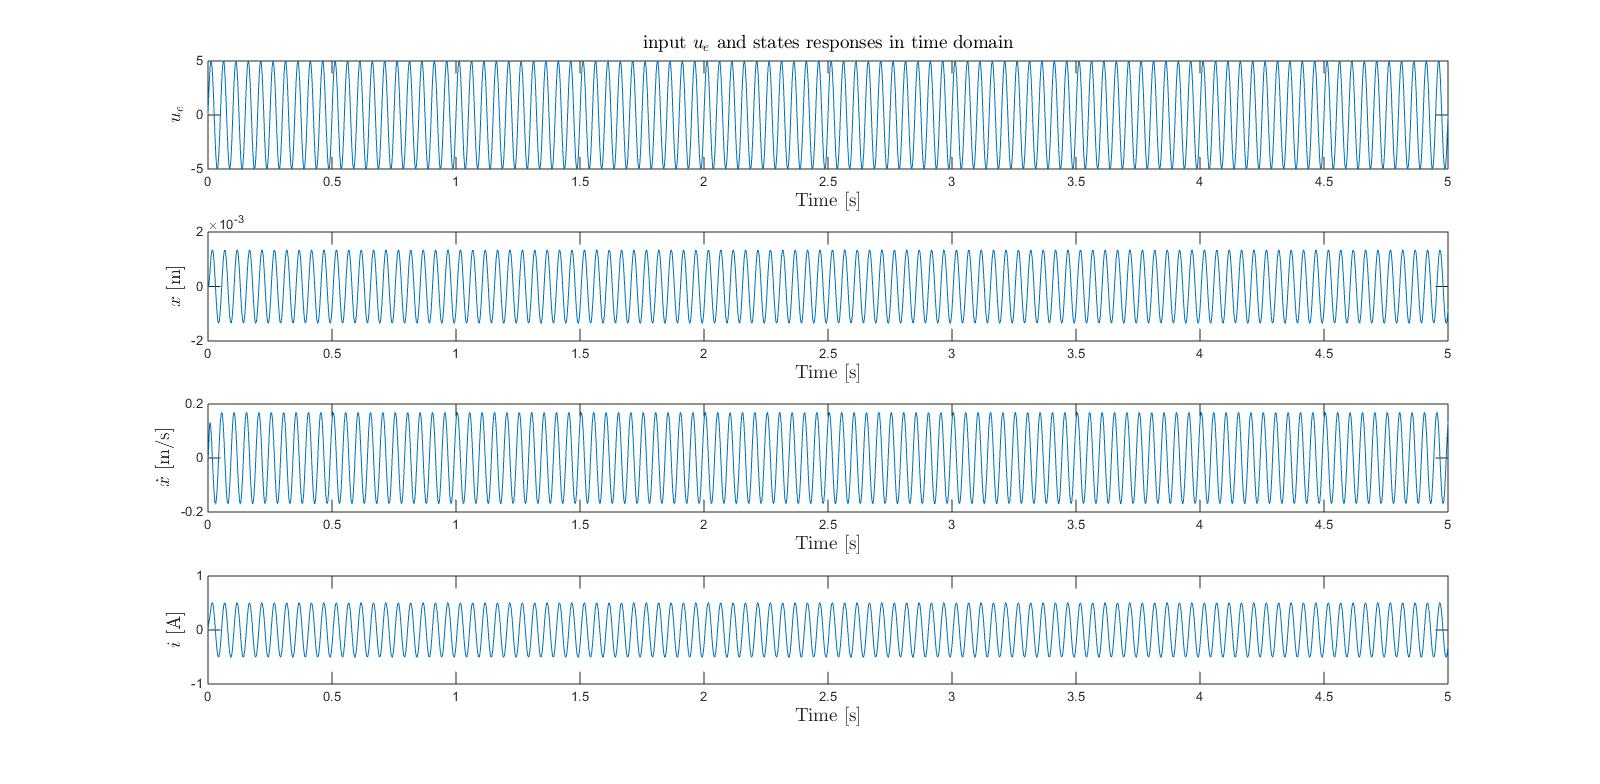
\includegraphics[scale=.3]{figures/responseLMt.jpg}
\caption{$u_e$ and states reponse to $u_e$ in time domain}
\label{fig:responseLMt}
\end{figure}
\begin{figure}[H]
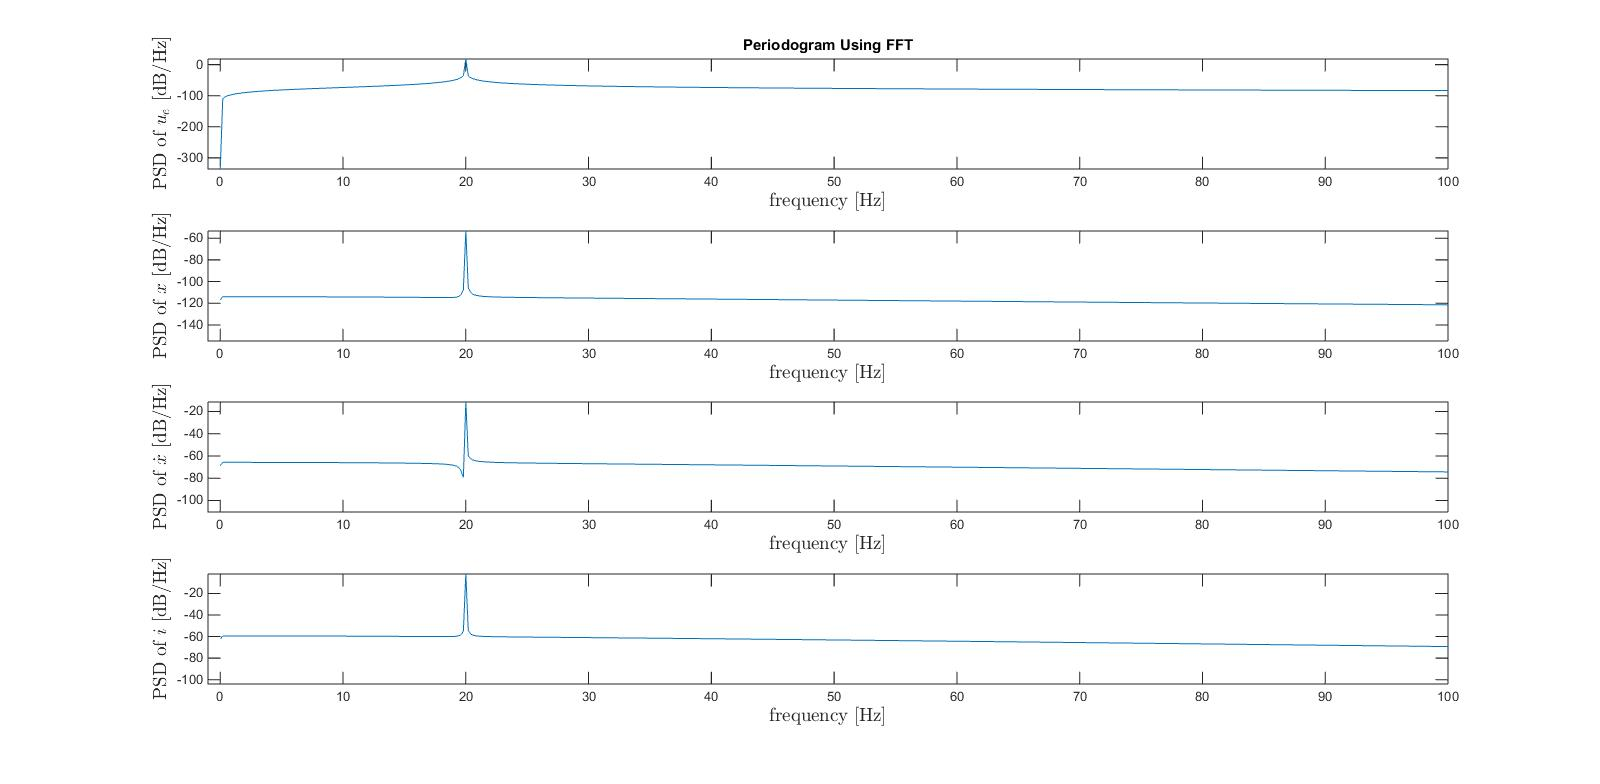
\includegraphics[scale=.3]{figures/responseLMf.jpg}
\caption{PSD of $u_e$ and states}
\label{fig:responseLMf}
\end{figure}

First, comparing the response to $u_e$ in the time domain (figure \ref{fig:responseNLMt} and figure \ref{fig:responseLMt}), the states response seems to be the same, but comparing the PSD of the states response (figure \ref{fig:responseNLMf} and figure \ref{fig:responseLMf}), we can see that the states response is not the same. Indeed, the linearised system is non affected by the harmonic distortion, there is only on frequency present in the state response, the one of 20$Hz$.
This result was expected because the nonlinear distortion only affects non-linear systems. Moreover, we have linearised the system with an input $u_e=0$ which means that we have a linearised system without harmonic, and then, we used a new input $u_e$ with a frequency $f_c=20Hz$, which means we only obtain a state response with an harmonic of a frequency of $f_c$.





